%!TEX root = ../thesis.tex

\chapter{Precision, Hardware, and Implementation Results}
\label{chap:variation-results}

Chapter~\ref{chap:mhd-validation-results} set the validation limits. This
chapter varies precision, build semantics, solver, device, resolution,
observation time, thread count, or CFL number in
Chapter~\ref{chap:methodology}'s matched groups.

\section{Deterministic output sensitivity}
\label{sec:ch5-deterministic-sensitivity}

\subsection{Euler--MHD cross-system sensitivity}
\label{sec:ch5-cross-system}

All sixteen Sod, LW3, Brio--Wu, and Orszag--Tang runs in
Figure~\ref{fig:ch5-cross-system} completed. Read in units of the binary32 unit
roundoff $u_{32}$, the O2-default fp32--fp64 mean-relative $L_1$ stays between
two and seven roundings, so in the domain mean the updates deliver about the
unit roundoff of the working precision and do not amplify it at these
resolutions \citep{higham_2002}. Amplification appears only in the absolute
$L_\infty$.

Where that maximum sits was measured rather than inferred.
Figure~\ref{fig:ch5-localisation} maps $|\rho_{32}-\rho_{64}|$ for matched
Orszag--Tang pairs at $256^2$. For HLLD the difference is strongly localised on
the shock and current-sheet network, $L_\infty/\text{mean}=2304$ with the top
$1\%$ of cells carrying $38\%$ of the total; for HLL the ratio is 12.5 and the
top $1\%$ carry $6\%$, close to diffuse. Concentration is therefore a solver
property, not one of the flow features alone.

\begin{figure}[htbp]
\centering
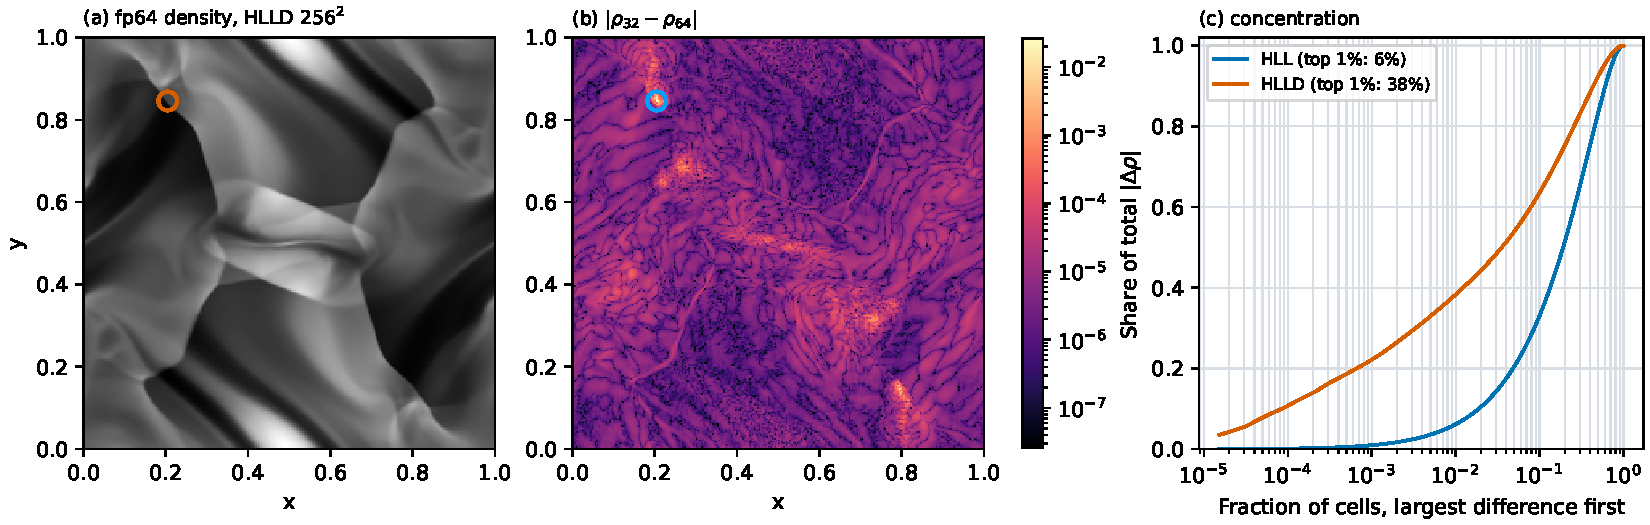
\includegraphics[width=\textwidth]{Figs/report2/ch5_precision_localisation}
\caption[Localisation of the precision discrepancy]{\textbf{Localisation of the
precision discrepancy.} Matched Orszag--Tang fp32/fp64 pairs at $256^2$, CPU.
(a) fp64 density with the $L_\infty$ cell circled; (b) the cellwise absolute
density difference on a log scale; (c) share of the total $|\Delta\rho|$
against the fraction of cells, largest first. HLL used CFL 0.4 and HLLD 0.2.}
\label{fig:ch5-localisation}
\end{figure}

% Source PDF SHA-256:
% 4a408e4e2e536e6478474022522c97785146ea966103f3cd208b4142372393e3
\begin{figure}[htbp]
\centering
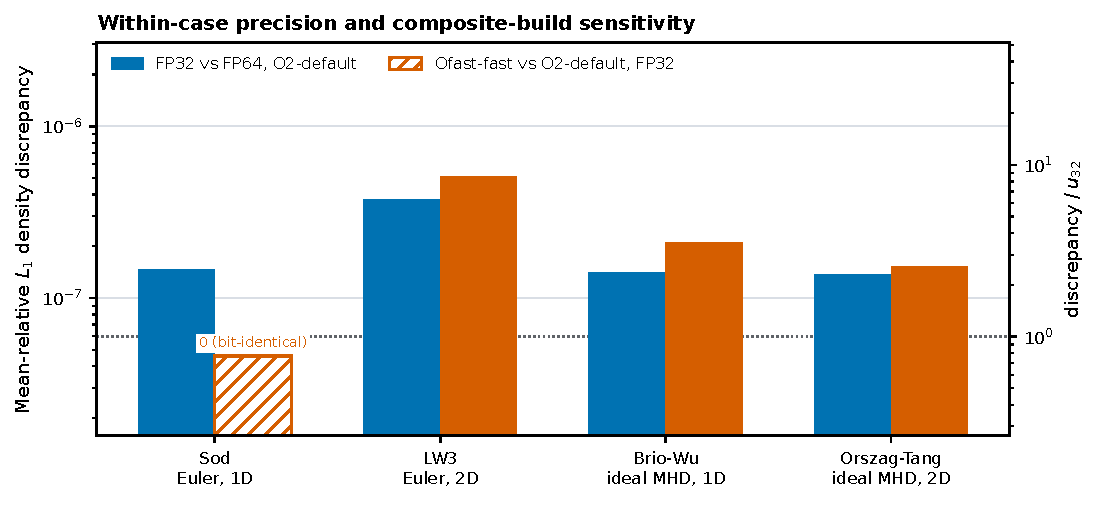
\includegraphics[width=\textwidth]{Figs/report2/ch5_cross_system_sensitivity}
\caption[Euler--MHD density sensitivity]{\textbf{Euler--MHD density
sensitivity.} Series: O2-default fp32 versus fp64 (precision); Ofast-fast
versus O2-default in fp32 (build pair). Only the fp32 build pair is plotted;
the fp64 build pair, between $4.24\times10^{-17}$ and $4.21\times10^{-16}$, is
reported in the text. LW3's $5.124\times10^{-7}$ bar is that fp32 build pair,
while Sod's is exactly zero and is annotated on a stub bar, since zero cannot
be placed on the log axis. In units of $u_{32}$ the precision series reads 2.46
(Sod), 6.31 (LW3), 2.35 (Brio--Wu) and 2.31 (Orszag--Tang), and the absolute
$L_\infty$ spans $3.837\times10^{-7}$--$5.254\times10^{-6}$. Grids are $N=200$
for Sod, $N=800$ for Brio--Wu, $200^2$ for LW3 and $128^2$ for Orszag--Tang.
Euler uses HLLC and MHD HLL.}
\label{fig:ch5-cross-system}
\end{figure}

A standalone $256^2$ Kelvin--Helmholtz comparison at $t=1.0$ and CFL 0.4 gave
$L_\infty$ of $1.786\times10^{-6}$ for HLL and $3.230\times10^{-6}$ for HLLD,
alongside the $1.075\times10^{-6}$ and $3.565\times10^{-6}$ of Brio--Wu and
Orszag--Tang. Every run completed with finite, positive states, so these
$10^{-6}$-scale local responses show sensitivity without precision-triggered
failure.

\subsection{Effective build-semantics sensitivity}
\label{sec:ch5-build-sensitivity}

The build pair in Figure~\ref{fig:ch5-cross-system} compared the O2-default
profile with Ofast-fast, which raises the optimisation level and relaxes
floating-point semantics together and so confounds the two. In fp64 the
mean-relative density response lay between $4.24\times10^{-17}$ and
$4.21\times10^{-16}$; in fp32 it ranged from exactly zero for Sod to
$5.124\times10^{-7}$ for LW3, exceeding that case's $3.762\times10^{-7}$
fp32--fp64 difference.

At $N=800$, $t=0.1$, CFL 0.4 and one thread, a Microsoft Visual C++
(MSVC)~19.51 Brio--Wu rebuild varied each axis separately
(Figure~\ref{fig:ch5-build-semantics}). All four /Ox--/O2
discrepancies were zero, so optimisation level alone left the output unchanged.
By contrast /fp:fast against compiler-default math
\citep{microsoftMsvcFp2021} gave $L_\infty$ values of $1.887\times10^{-15}$ and
$1.311\times10^{-6}$ for HLL and $4.413\times10^{-15}$ and
$1.729\times10^{-6}$ for HLLD, in fp64 and fp32, the larger fp32 response
following its coarser unit roundoff. Changing $\leq$ to $<$ gave zero for both
HLL groups but $3.886\times10^{-15}$ and $2.608\times10^{-6}$ for HLLD. The HLL
zero is structural, since the clamp forces $S_L^{H}<0<S_R^{H}$ so that neither
outer dispatch branch can be selected (Section~\ref{sec:ch2-riemann}), whereas
HLLD keeps the unclamped Davis speeds and three further ties at $S_L^*$,
$S_R^*$ and $S_M$, across each of which the flux is value-continuous. The
variants therefore diverge only where rounding decides the side of an exact
zero.

Moving only the MSVC baseline instruction set from /arch:SSE2 to /arch:AVX2
left all four solver--precision groups bitwise identical although the binaries
differed by hash: widening the vector registers changed the generated code but
not the arithmetic, since /fp:precise forbids the reassociation they would
otherwise invite.

\begin{figure}[htbp]
\centering
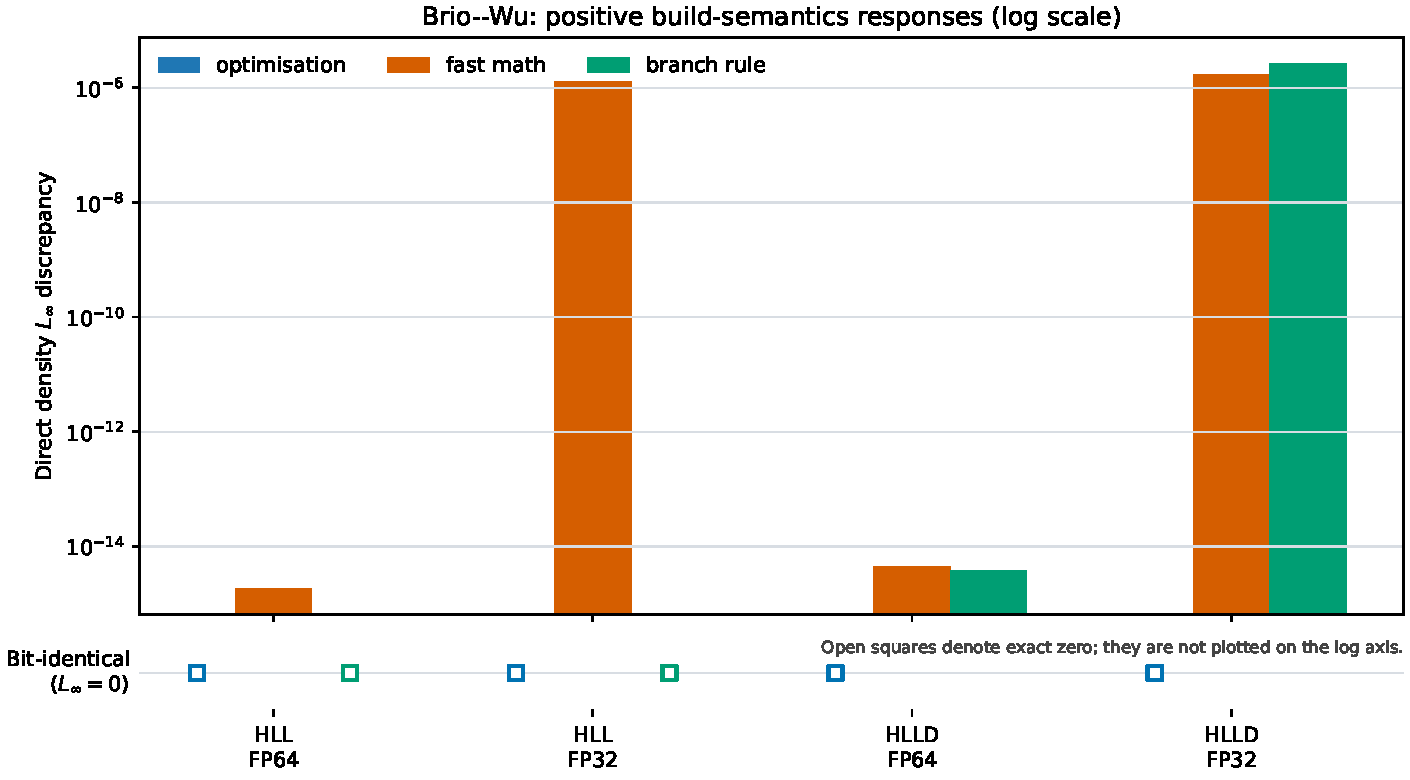
\includegraphics[width=\textwidth]{Figs/report2/ch5_build_semantics}
\caption[Isolated Brio--Wu build-semantics response]{\textbf{Isolated
Brio--Wu build-semantics response.} Direct density $L_\infty$ responses to one
MSVC~19.51 axis change at $N=800$, $t=0.1$. Positive log bars show discrepancy,
not accuracy; exact zeros occupy the separate Bit-identical ($L_\infty=0$)
marker row.}
\label{fig:ch5-build-semantics}
\end{figure}

\section{Solver and device performance}
\label{sec:ch5-performance}

\subsection{CPU timing: HLL versus HLLD}
\label{sec:ch5-solver-timing}

Figure~\ref{fig:ch5-kh-timing} compares CPU cost within a fixed $256^2$
Kelvin--Helmholtz configuration at $t=1.0$, CFL 0.4 and
\texttt{OMP\_NUM\_THREADS}=1, all groups taking 1148 steps. A fixed-width
vector register holds twice as many fp32 as fp64 values, yet the fp32 speed-ups
stay well below $2\times$, and HLLD's 15--17\% premium is modest despite three
extra waves and fourteen guards per interface: both point away from an
arithmetic-throughput limit \citep{williamsEtAl2009roofline}.

% Source PDF SHA-256:
% 12e0140c6302bbbcd98ce8845c2a46a483c6632dcadcf598b7f2cf09fea85358
\begin{figure}[htbp]
\centering
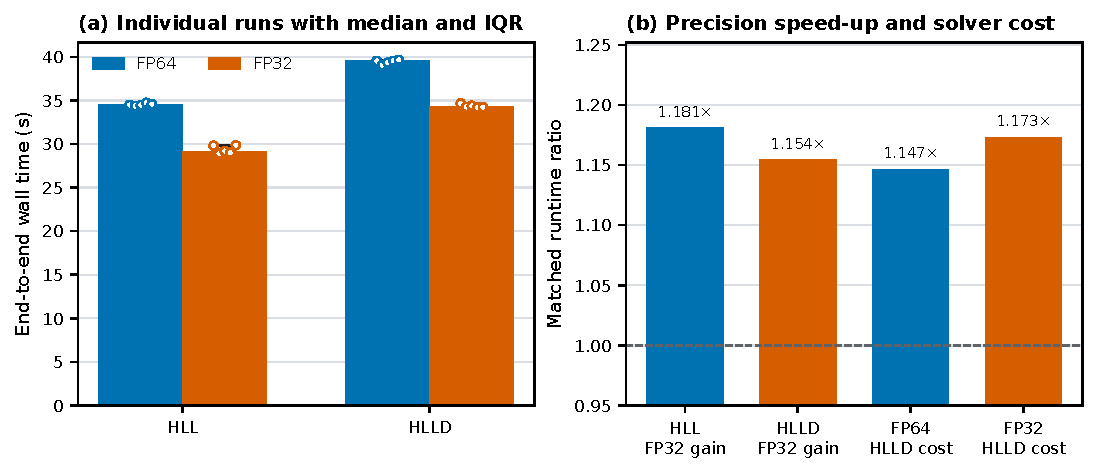
\includegraphics[width=\textwidth]{Figs/report2/ch5_kh_timing}
\caption[KH solver and precision timing]{\textbf{KH solver and precision
timing.} Median and IQR of $n=5$ subprocess wall times after one excluded CPU
warm-up per group. Runs used $256^2$, $t=1.0$, CFL 0.4, and
\texttt{OMP\_NUM\_THREADS}=1. The fp64 medians were 34.484~s for HLL and
39.542~s for HLLD and the fp32 medians 29.196~s and 34.254~s, so fp32 was
$1.181\times$ and $1.154\times$ faster while HLLD cost $1.147\times$ HLL in
fp64 and $1.173\times$ in fp32. All 20 outputs had zero within-group ULP drift;
these are cost and repeatability results.}
\label{fig:ch5-kh-timing}
\end{figure}

\subsection{Matched CPU/GPU agreement and performance}
\label{sec:ch5-hardware}

The same-precision CPU/GPU saved states in Table~\ref{tab:ch4-cpu-gpu} were
bit-identical in both maximum ULP and absolute $L_\infty$, and the $n=5$ groups
in Figure~\ref{fig:ch5-hardware} reproduce that result. Since one device flag
arranges it, that flag was varied: rebuilding only the CUDA kernel translation
unit with nvcc's default \texttt{--fmad=true}, holding host binary, case, grid,
precision and update order fixed, removed bitwise agreement in all four pairs. The density
$L_\infty$ differences were $1.665\times10^{-15}$ and $2.309\times10^{-14}$ in
fp64 for Brio--Wu and Orszag--Tang, and $2.265\times10^{-6}$ and
$2.074\times10^{-5}$ in fp32. The Brio--Wu fp32 value shares its case, grid,
solver and final time with two axes already reported, and exceeds both: the
$1.075\times10^{-6}$ fp32--fp64 difference and the $1.311\times10^{-6}$
/fp:fast response. On that workload one device compiler default moved the
stored field further than halving the working precision did.

Contraction is only part of nvcc's relaxed-math setting, so a third column
rebuilt the same kernels with \texttt{--use\_fast\_math}, which also enables
flush-to-zero, approximate division and square root, and fast intrinsics. In
fp64 it reproduced the contraction column exactly, its single-precision
intrinsics not applying; in fp32 it gave $1.431\times10^{-6}$ and
$1.574\times10^{-5}$, both \emph{below} the contraction-only response. The more
relaxed build therefore sat closer to the host baseline, so these
transformations partly cancel rather than accumulate.

Median wall-time ratios show a crossover, the GPU being slower for $800\times1$
Brio--Wu but about $6\times$ faster for $256^2$ Orszag--Tang. The CPU side is a
single-core execution, since the MHD sweeps carry no work-sharing directives
(Section~\ref{sec:ch2-execution}), so one core of a 24-core part is set against
the whole device: these ratios bound a serial-to-device gain rather than a
processor comparison, and a work-shared host would close much of it.

Brio--Wu's small workload leaves little useful device work, so context
creation, kernel launches, transfers and output dominate, whereas the larger
Orszag--Tang mesh amortises those fixed costs. In end-to-end cell updates per
second, portable across machines in a way seconds are not, the CPU delivered
2.1--4.1 million across both workloads while the GPU spanned 0.22 to 15.1
million, a seventyfold range on one kernel. GPU fp64/fp32 median ratios of
$1.146\times$ and $1.260\times$ are far below the fp64 penalty a consumer
device imposes, again placing the kernel away from a floating-point bound.

% Source PDF SHA-256:
% 643820272d5a8cedc0ca6235a280b66d751fc4764fe65b80fe6c13ad470aba7c
\begin{figure}[htbp]
\centering
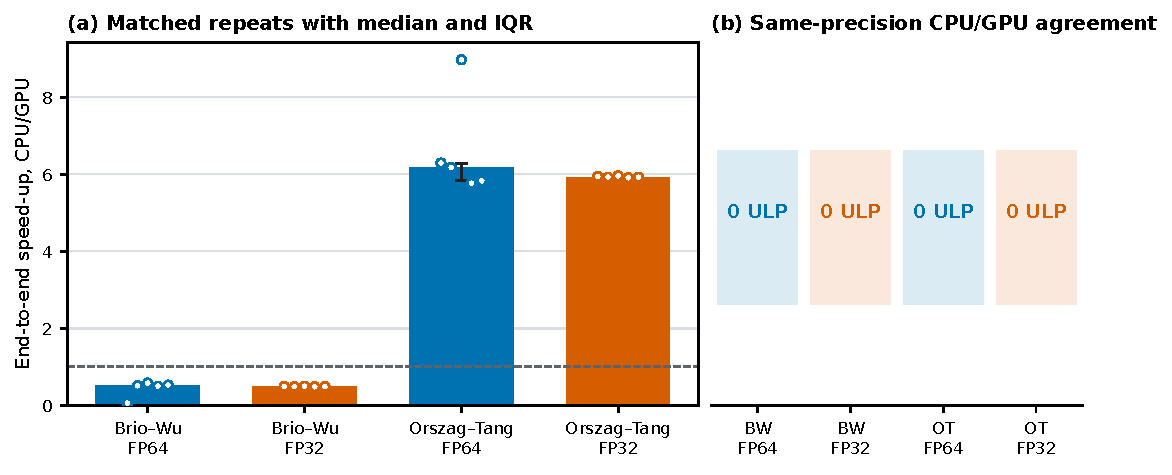
\includegraphics[width=\textwidth]{Figs/report2/ch5_hardware_reproducibility}
\caption[Repeated CPU/GPU agreement and timing]{\textbf{Repeated CPU/GPU
agreement and timing.} Median, IQR and all $n=5$ CPU/GPU wall-time ratios for
HLL Brio--Wu ($800\times1$) and Orszag--Tang ($256^2$) in fp64 and fp32. The
CPU baseline is single-core, as the MHD path has no work sharing, so these are
serial-host ratios. The agreement panel reports the maximum same-precision ULP
difference; all GPU repeats were retained.}
\label{fig:ch5-hardware}
\end{figure}

\section{Scale, time, and stochastic sensitivity}
\label{sec:ch5-scale-time-stochastic}

\subsection{Resolution dependence of discrepancies}
\label{sec:ch5-resolution-precision}

All eight self-refinement groups completed, and in every one the density
mean-$L_1$ precision discrepancy $D_N$, and therefore
$S_N=D_N/E^{64}_{256,512}$, rose monotonically from $128^2$ to $512^2$
(Figure~\ref{fig:ch5-precision-refinement}).
Refinement at fixed CFL takes more steps per unit of simulated time and
resolves thinner Orszag--Tang (OT) current sheets and sharper
Kelvin--Helmholtz (KH) shear gradients. Even so the largest value,
$S_{512}=2.76\times10^{-2}$ for KH--HLLD, stayed below 3\% of the matched fp64
finest adjacent-grid difference, while the largest local response, OT--HLLD at
$512^2$, reached $L_\infty=5.031\times10^{-2}$ against a mean-$L_1$ of
$5.554\times10^{-5}$.

In units of $u_{32}$ the domain-mean discrepancy rises from 2.31 to 54.84 for
OT/HLL and from 12.96 to 335.46 for OT/HLLD, so the few-roundings reading of
Section~\ref{sec:ch5-cross-system} is a coarse-grid statement: refinement
amplifies round-off in the domain mean, not only locally. Three grids cannot
fix the rate, and the OT/HLL trend is dominated by one factor-11.5 jump between
$256^2$ and $512^2$, so no crossover grid is extrapolated. The HLLD entries
describe HLLD itself, its per-line fallback having fired twice in over three
million line updates at $512^2$ (Section~\ref{sec:ch4-orszag-tang}).

% Source PDF SHA-256:
% 51ad93f4fd9ebba37fe868da105e360a29785b82dd7faf57af2a6d001914c68c
\begin{figure}[htbp]
\centering
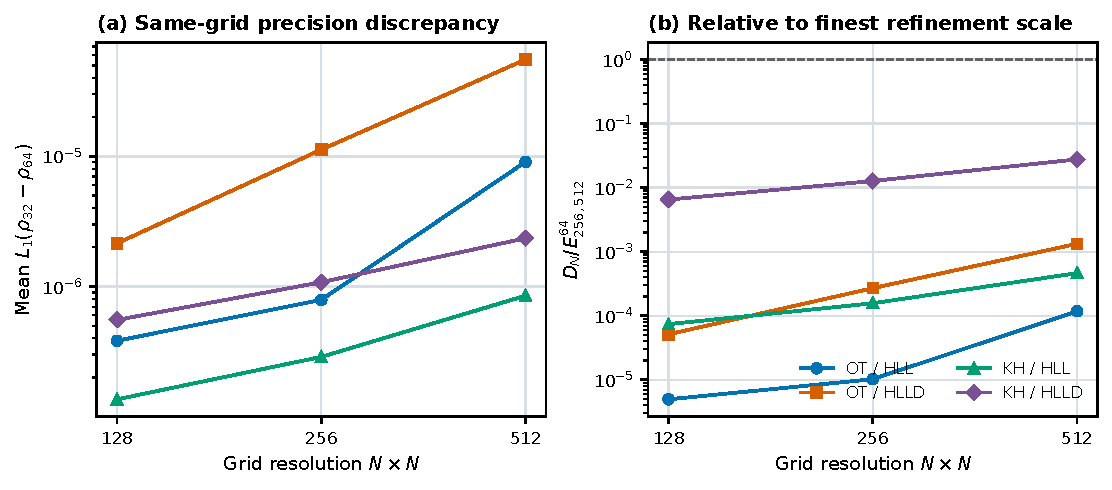
\includegraphics[width=\textwidth]{Figs/report2/ch5_precision_refinement_context}
\caption[Precision discrepancy relative to refinement scale]{\textbf{Precision
discrepancy relative to refinement scale.} (a) Same-grid fp32--fp64 density
mean-$L_1$, $D_N$, for OT and KH with HLL/HLLD at $128^2$, $256^2$ and
$512^2$. (b) $S_N=D_N/E^{64}_{256,512}$ using the matched fp64 adjacent-grid
difference. OT used $t=0.5$ and KH $t=1.0$; HLL used CFL 0.4 and HLLD 0.2.}
\label{fig:ch5-precision-refinement}
\end{figure}

\subsection{Growth of discrepancies with time}
\label{sec:ch5-temporal}

The temporal test fitted both models of Equation~\ref{eq:ch3-temporal-fit} to
the CPU HLL density discrepancies of Figure~\ref{fig:ch5-temporal} over the
fixed windows $[0.01,0.1]$ and $[0.1,0.5]$. On Brio--Wu the exponential gave
$\lambda=30.6153$ with root-mean-square log residual 0.143, predicting
$\exp(\lambda\Delta t)\simeq16$ across the window against an endpoint ratio of
about 24. Fitted to the same 13 samples, the power law gave $k=1.44$ with
residual 0.064 and $R^2=0.993$ against 0.963, halving both the typical and the
worst log-space departure. The $L_\infty$ series barely separates the models,
0.172 against 0.186.

In units of $u_{32}$ the Brio--Wu mean discrepancy rises from 0.098 at
$t=0.01$ to 2.351 at $t=0.1$, whereas Orszag--Tang already stands at 1.756 at
its first sample and stays between about 2.1 and 2.6 thereafter, so any earlier
rise went unobserved. Both arrive at about 2.3 roundings at the resolutions
used, and the apparent reversal, a one-dimensional shock tube separating faster
than a chaotic two-dimensional case, records where each series was sampled
relative to that level rather than anything about dimensionality.
Orszag--Tang's near-zero slopes sit against RMS log residuals of 0.039 and
0.201, so its mean series is a tight plateau while its maximum is scattered,
and that level does not survive refinement
(Section~\ref{sec:ch5-resolution-precision}).

Precision is not the only axis that grows. The same treatment was applied to
two build axes on the identical Brio--Wu fp32 configuration, each stopping time
again an independently executed pair (Figure~\ref{fig:ch5-impl-temporal}).
Relaxed host math grew from $4.610\times10^{-9}$ to $1.176\times10^{-7}$ in
density mean $L_1$ over $t\in[0.01,0.1]$ and device contraction from
$2.990\times10^{-9}$ to $1.058\times10^{-7}$, both rising from about a tenth of
a rounding to roughly 3.2--3.5 in units of $u_{32}$. Power laws again fit
better, at $k=1.39$ with $R^2=0.986$ for the host axis and $k=1.57$ with
$0.993$ for the device axis, against $0.950$ and $0.921$ for the exponentials.
All three axes therefore accumulate at a similar rate, $k\simeq1.4$--$1.6$.

\begin{figure}[htbp]
\centering
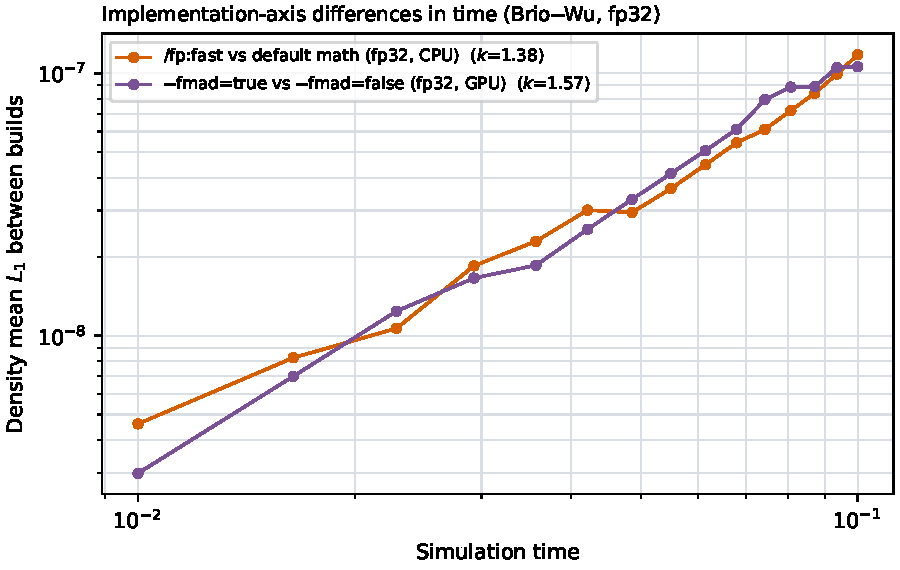
\includegraphics[width=0.72\textwidth]{Figs/report2/ch5_implementation_temporal}
\caption[Implementation-axis differences in time]{\textbf{Implementation-axis
differences in time.} Density mean $L_1$ between two builds differing in one
declared axis, Brio--Wu fp32, $N=800$, HLL, CFL 0.4, at 15 independently
executed stopping times. Fitted power-law exponents $k$ are shown.}
\label{fig:ch5-impl-temporal}
\end{figure}

The exponential model is imported from the perturbation-growth picture for
chaotic systems \citep{lorenz1963}, in which a difference grows like
$\mathrm{e}^{\lambda t}$ only while it stays small
\citep{boffettaEtAl2002predictability}. Here it is the weaker description on
every axis measured. Brio--Wu is not
chaotic, and $k=1.44$ places its mean discrepancy on a power law in the step
count: faster than the $k=0.5$ of an incoherent random walk and than the
$k=1$ of coherent per-step addition, so accumulation is mildly reinforced,
but nowhere near amplification. The fitted $\lambda$ therefore carries no
e-folding interpretation, and quoting it alone would overstate the mechanism.

% Source PDF SHA-256:
% 0cb7a079c9afdde10f3e78d3d65d123a3346ba8fdbb692ec335e74c1e81de024
\begin{figure}[htbp]
\centering
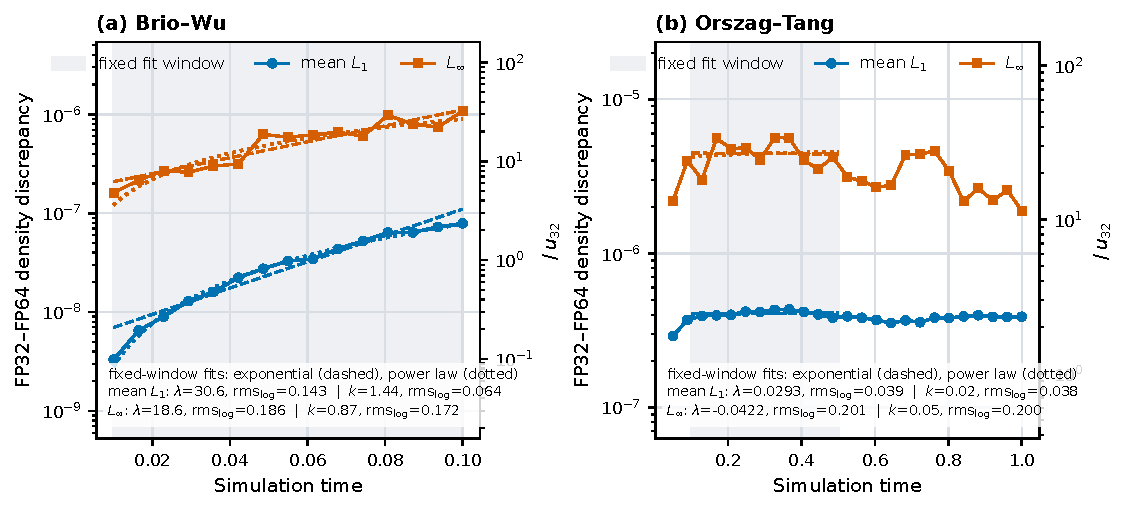
\includegraphics[width=\textwidth]{Figs/report2/ch5_temporal_discrepancy}
\caption[Fixed-window fp32--fp64 temporal discrepancy]{\textbf{Fixed-window
fp32--fp64 temporal discrepancy.} Density mean $L_1$ and $L_\infty$ from 15
aligned Brio--Wu pairs and 25 aligned Orszag--Tang pairs, the latter running
from $t=0.05$; the fixed $[0.01,0.1]$ and $[0.1,0.5]$ fitting windows retain 13
and 10 positive observations, so the Orszag--Tang window opens after that
series begins. CPU HLL at $N=800$ and $128^2$. Dashed lines are the
exponential fit with inverse-time slope $\lambda$, dotted lines the power law
with exponent $k$, fitted to identical samples. The right-hand $u_{32}$ axis
normalises by the reference field mean and so is defined for the mean-$L_1$
series; the absolute $L_\infty$ series is read on the left axis only.}
\label{fig:ch5-temporal}
\end{figure}

\subsection{Monte Carlo arithmetic}
\label{sec:ch5-mca}

Verificarlo instrumentation \citep{denis_etal_2016} supplied the MCA
runs, randomly rounding each operation at a chosen virtual precision after
\citet{parker_1997}. The solver was rebuilt whole-program with
\texttt{verificarlo-c++}, so operations in its own translation units are
perturbed and library calls are not.
Table~\ref{tab:ch5-mca-primary} retains the matched Brio--Wu density
results at $N=800$, $t=0.1$, with 30 samples for each of HLL and HLLD. At
virtual p24, the maximum cellwise sample standard deviations were
$2.275\times10^{-6}$ and $4.007\times10^{-6}$; the corresponding deterministic
fp32--fp64 $L_\infty$ differences were $1.075\times10^{-6}$ and
$1.629\times10^{-6}$. Their quotients are 2.12 and 2.46.

The two statistics are not equivalent, but their order-one quotients place the
deterministic fp32--fp64 separation on the scale of the cloud from random
24-bit rounding, so a single fp32 endpoint undersamples rounding sensitivity.
At virtual p53 the spreads fell to $5.117\times10^{-15}$ and
$8.442\times10^{-15}$, eight to nine orders below p24. No confidence interval
is attached to these $n=30$ spreads \citep{sohier_etal_2021}.

\begin{table}[htbp]
\centering
\small
\begin{tabularx}{\textwidth}{@{}lrrrrX@{}}
\toprule
Solver & Deterministic $L_\infty$ & p53 spread & p24 spread & p24/$L_\infty$ & Scope \\
\midrule
HLL  & $1.075\times10^{-6}$ & $5.117\times10^{-15}$ & $2.275\times10^{-6}$ & 2.12 & $N=800$, $t=0.1$, 30 samples \\
HLLD & $1.629\times10^{-6}$ & $8.442\times10^{-15}$ & $4.007\times10^{-6}$ & 2.46 & $N=800$, $t=0.1$, 30 samples \\
\bottomrule
\end{tabularx}
\caption[Matched Brio--Wu deterministic and MCA scales]{\textbf{Matched
Brio--Wu deterministic and MCA scales.} Deterministic $L_\infty$ is the
fp32--fp64 density difference; MCA spread is the maximum cellwise sample
standard deviation. Their ratio is descriptive because the statistics are not
equivalent. Virtual p24 and p53 are not IEEE fp32 and fp64.}
\label{tab:ch5-mca-primary}
\end{table}


\section{Robustness checks}
\label{sec:ch5-robustness}

\subsection{Requested-thread null control and CFL sensitivity}
\label{sec:ch5-thread-cfl}

As Section~\ref{sec:ch2-execution} establishes, the MHD sweeps carry no
work-sharing directives and their only reduction is an exactly associative
maximum, so requested counts of 1, 2, 4 and 8 could not change the result and
did not: all matched the one-thread Orszag--Tang and KH states at zero ULP. The
non-determinism reported for parallel summation \citep{collange_etal_2015}
needs a summation reduction, which this scheme carries only in diagnostics.

All KH runs at CFL 0.2, 0.4, 0.6, and 0.8 completed with finite, positive
states, and Figure~\ref{fig:ch5-kh-cfl} shows the fp32--fp64 density
$L_\infty$ separation falling as CFL rises: for HLL by 5.25 between 0.2 and
0.8, against a fourfold drop in step count. Lower CFL offers more rounding
opportunities, but the separation follows no simple accumulation law, since
5.25 exceeds the fourfold drop of coherent per-step addition and far exceeds
the twofold change of a $\sqrt{n}$ random walk. Two features stop that excess
being read as a mechanism: CFL 0.6 sits out of order in both solvers,
indistinguishable from scatter at one run per setting, and changing CFL changes
the fp64 solution too, so each point differences a different matched pair.
Refinement rates proved insensitive to the same setting
(Section~\ref{sec:ch4-orszag-tang}).

\begin{figure}[htbp]
\centering
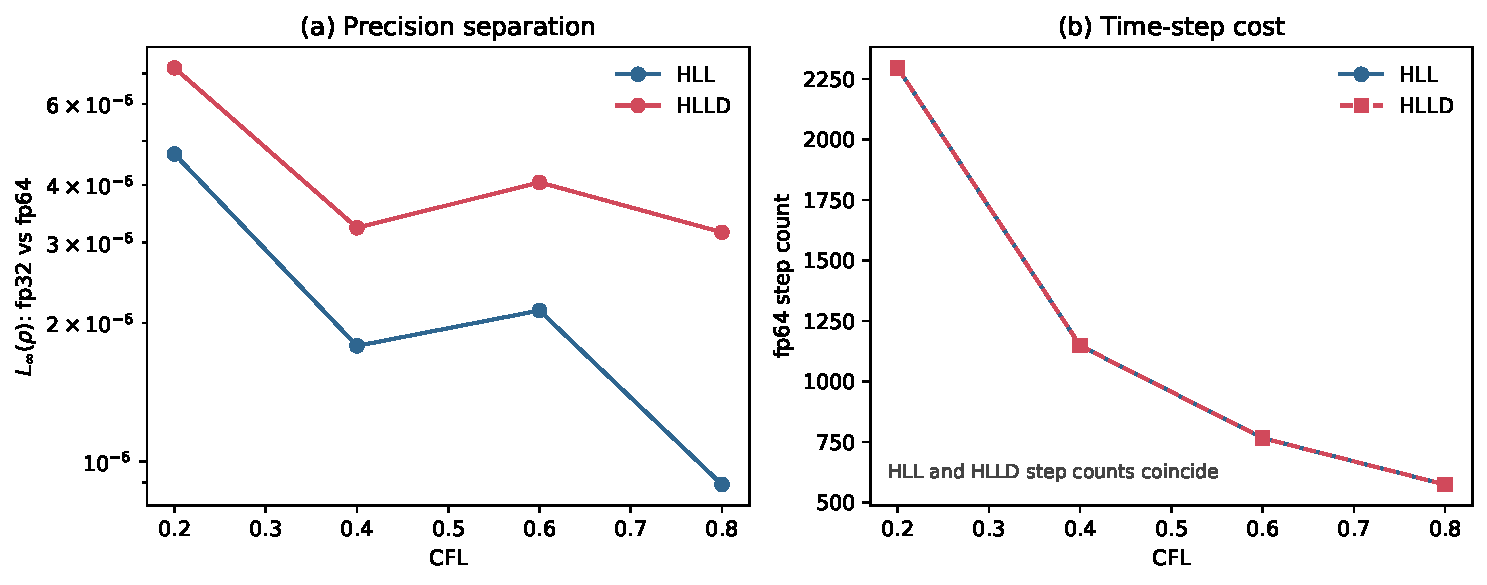
\includegraphics[width=\textwidth]{Figs/report2/ch5_kh_cfl}
\caption[Kelvin--Helmholtz CFL sensitivity]{\textbf{Kelvin--Helmholtz CFL
sensitivity.} Density fp32--fp64 $L_\infty$ and fp64 step count for HLL and
HLLD at $256^2$, $t=1.0$. The precision response falls as CFL rises and the
step count drops, with CFL 0.6 out of order in both solvers.}
\label{fig:ch5-kh-cfl}
\end{figure}

Every discrepancy, separation and growth reported in this chapter is the
difference between two runs of the same solver on the same grid, differing only
in the declared axis: not a physical growth, not an instability, and not an
error against a reference solution.
